\documentclass[12pt,a4paper]{article}

\makeatletter
    \input{../config/header[fr].sty}

    \usepackage{01-tables}
\makeatother

\usepackage{amsmath}


\begin{document}

\section{OK}

\subsection{Commentaires}


\begin{tikzpicture}
    \tkzTabInit{
        Comment     / 1   ,
        Comment Bis / 1.5
    }{ , }
    
% COMMENTS
    \comLine      {0}{Commentaire par défaut}
    \comLine[gray]{1}{Commentaire gris}
\end{tikzpicture}


% ------------------ %


\subsection{Affines}

\begin{tikzpicture}
    \tkzTabInit{
        Line ap  / 1.5 ,
        Line an  / 1.5
    }{ , }

% LINES
    \graphSign[purple]{0}{ax+b, ap}{r}
    \graphSign        {1}{ax+b, an}{r}
\end{tikzpicture}


% ------------------ %


\subsection{2nd degré}

\begin{tikzpicture}
    \tkzTabInit{
        Parabola ap dp / 1.5 ,
        Parabola an dp / 1.5 ,
        %
        Parabola ap dz / 1.5 ,
        Parabola an dz / 1.5 ,
        %
        Parabola ap dn / 1.5 ,
        Parabola an dn / 1.5
    }{ , }
    
% PARABOLAS  delta > 0
    \graphSign[red]  {0}{ax2+bx+c, ap, dp}{r1}{r2}
    \graphSign[black]{1}{ax2+bx+c, an, dp}{r1}{r2}

% PARABOLAS  delta = 0
    \graphSign[gray]{2}{ax2+bx+c, ap, dz}{r}
    \graphSign      {3}{ax2+bx+c, an, dz}{r}

% PARABOLAS  delta < 0
    \graphSign[orange]{4}{ax2+bx+c, ap, dn}
    \graphSign        {5}{ax2+bx+c, an, dn}
\end{tikzpicture}


% ------------------ %


\subsection{Fonctions de réf.}

\begin{tikzpicture}
    \tkzTabInit{
        $x^2$      / 1.5 ,
        $\sqrt{x}$ / 1.5 ,
        $\frac1x$  / 1.5 ,
        $|x|$      / 1.5 ,
        $\exp(x)$  / 1.5 ,
        $\ln(x)$   / 1.5
    }{ , }
    
% REFERENCE FUNCTIONS
    \graphSign[red]           {0}{x2}
    \graphSign                {1}{sqrt}
    \graphSign[black]         {2}{1/x}
    \graphSign[green!40!black]{3}{abs}
    
    \graphSign[orange]         {4}{exp}
    \graphSign[yellow!30!green]{5}{ln}
\end{tikzpicture}
\end{document}
